%%%%%%%%%%%%%%%%%%%%%%%%%%%%%%%%%%%%%%%%%%%%%%%%%%%%%%%%%%%%%%%%%%%%%%%%%%%%%%%%
%2345678901234567890123456789012345678901234567890123456789012345678901234567890
%        1         2         3         4         5         6         7         8

\documentclass[letterpaper, 10 pt, conference]{ieeeconf}  % Comment this line out if you need a4paper

%\documentclass[a4paper, 10pt, conference]{ieeeconf}      % Use this line for a4 paper

% \IEEEoverridecommandlockouts                              % This command is only needed if
                                                          % you want to use the \thanks command

\overrideIEEEmargins                                      % Needed to meet printer requirements.

%In case you encounter the following error:
%Error 1010 The PDF file may be corrupt (unable to open PDF file) OR
%Error 1000 An error occurred while parsing a contents stream. Unable to analyze the PDF file.
%This is a known problem with pdfLaTeX conversion filter. The file cannot be opened with acrobat reader
%Please use one of the alternatives below to circumvent this error by uncommenting one or the other
%\pdfobjcompresslevel=0
%\pdfminorversion=4

% See the \addtolength command later in the file to balance the column lengths
% on the last page of the document

% The following packages can be found on http:\\www.ctan.org
\usepackage{graphicx} % for pdf, bitmapped graphics files
%\usepackage{epsfig} % for postscript graphics files
%\usepackage{mathptmx} % assumes new font selection scheme installed
%\usepackage{times} % assumes new font selection scheme installed
\usepackage{amsmath} % assumes amsmath package installed
\usepackage{amssymb}  % assumes amsmath package installed
%\usepackage{dsfont}
\usepackage{algorithm}
\usepackage{algorithmic}
\usepackage{commath}

\usepackage{xcolor}
\newcommand{\todo}[1]{{\color{blue}[TODO: #1]}}
\newcommand{\response}[1]{{\color{green}[RESPONSE: #1]}}
\graphicspath{{figures/}}


\DeclareMathOperator*{\argmax}{arg\,max}
\DeclareMathOperator*{\argmin}{arg\,min}

\title{\LARGE \bf
Multi-Agent Autonomous Mapping of Unknown GPS-Denied Environments Using a Relative Navigation Framework}

\author{Jacob M. Olson$^{1}$, Timothy W. McLain$^{2}$ \todo{include Matthiew Labbe?}% <-this % stops a space
%\thanks{This research was supported through the Center for Unmanned Aircraft Systems (C-UAS), a National Science Foundation-sponsored industry/university cooperative research center (I/UCRC) under NSF Award No. IIP-1650547 along with significant contributions from C-UAS industry members.}% <-this % stops a space
\thanks{$^{1}$The corresponding author can be contacted at
        {\tt\small jacobmo at byu.edu}.}%
\thanks{$^{2}$All authors are with the Department of Mechanical Engineering or Electrical and Computer Engineering,
        Brigham Young University, Provo, UT, 84602, USA.}%
%\thanks{$^{3}$C. Peterson is with the Faculty of Electrical and Computer Engineering,
%		Brigham Young University, Provo, UT, 84602, USA.
%        {\tt\small cammy.peterson at byu.edu}}%
%\thanks{$^{4}$R. W. Beard is with the Faculty of Electrical and Computer Engineering,
%		Brigham Young University, Provo, UT, 84602, USA.
%        {\tt\small beard at byu.edu}}%
}

\begin{document}

\maketitle
\thispagestyle{empty}
\pagestyle{empty}


%%%%%%%%%%%%%%%%%%%%%%%%%%%%%%%%%%%%%%%%%%%%%%%%%%%%%%%%%%%%%%%%%%%%%%%%%%%%%%%%
\begin{abstract}

\todo{When generating 3D maps with unmanned aerial vehicles (UAVs), it is important for the mapping algorithm to have good coverage of the environment. It is also important, especially when planning paths for multiple agents, to have loop closures along each flight path and with other agents. Because multirotor UAVs are limited in flight time, the flight paths must be limited in length. Generating a good flight path to map a new environment can be difficult and tedious because of the free-form nature of a flight path. To solve this problem, we propose using a genetic algorithm designed to maximize total area coverage while minimizing flight time and enforcing sufficient loop closures. The natural ability of genetic algorithms to rapidly explore a design space is advantageous when solving complex free-form problems like path planning.}

\end{abstract}


%%%%%%%%%%%%%%%%%%%%%%%%%%%%%%%%%%%%%%%%%%%%%%%%%%%%%%%%%%%%%%%%%%%%%%%%%%%%%%%%
\section{Introduction}

The remainder of the paper is organized as follows: Section \ref{approach} describes framework used to map the environment and background on what previous work has made this research possible. Section \ref{planning} details the planning and control schemes used to successfully navigate the unknown area. Then method used to combine maps of multiple agents are then explained in Section \ref{merge}. Results showing and evaluating the generated maps are presented in Section \ref{results}. Finally, conclusions are presented in Section \ref{conclusions}.

%%%%%%%%%%%%%%%%%%%%%%%%%%%%%%%%%%%%%%%%%%%%%%%%%%%%%%%%%%%%%%%%%%%%%%%%%%%%%%%%
\section{Technical Approach}\label{approach}

\subsection{Problem Statement}

The goal of

\subsection{Sensors}

Since we are operating in a GPS-denied environment, we are not able to rely on GPS measurements to give us global information about where the UAVs are located. As shown in Fig. \ref{fig:rtab_network} the sensors used by the UAV to estimate its state are an RGB-D camera, a planar laser scanner, a LiDAR pencil-beam sensor and an IMU on the onboard flight controller. \todo{how much do I talk about sensors here?}

\subsection{Estimation}

Estimation is the most critical element in enabling autonomous flight. Without good position and attitude estimation, autonomous navigation algorithms are unable to

\subsubsection{RTAB-Map}

RTAB-Map is a powerful open source library that uses graph-based SLAM with appearence based loop closures to generate high-quality, dense 3D maps of environments without the use of GPS. As part of this is able to accurately estimate position within the map with little error. This has been extended to work with multi-session mapping, but currently not simultaneous multi-agent mapping. This paper proposes a method to extend the functionality of RTAB-Map to combine the maps of multiple agents into a single map in near real time.

RTAB map does not estimate the attitude of a UAV with enough frequency to autonomously navigate so we used the relative navigation framework to estimate attitude and relative state.

\subsubsection{RMEKF}
the RMEKF was shown to successfully estimate the UAV's state sufficient to autonomously navigate in GPS-denied environments that had been previously mapped, but has thus far not been extended to estimation and navigation in unknown and unmapped environments, this paper proposes a method to extend the functionality to these environments.

\subsection{Control}
\subsection{Inputs/Outputs}

\begin{figure*}
\centering
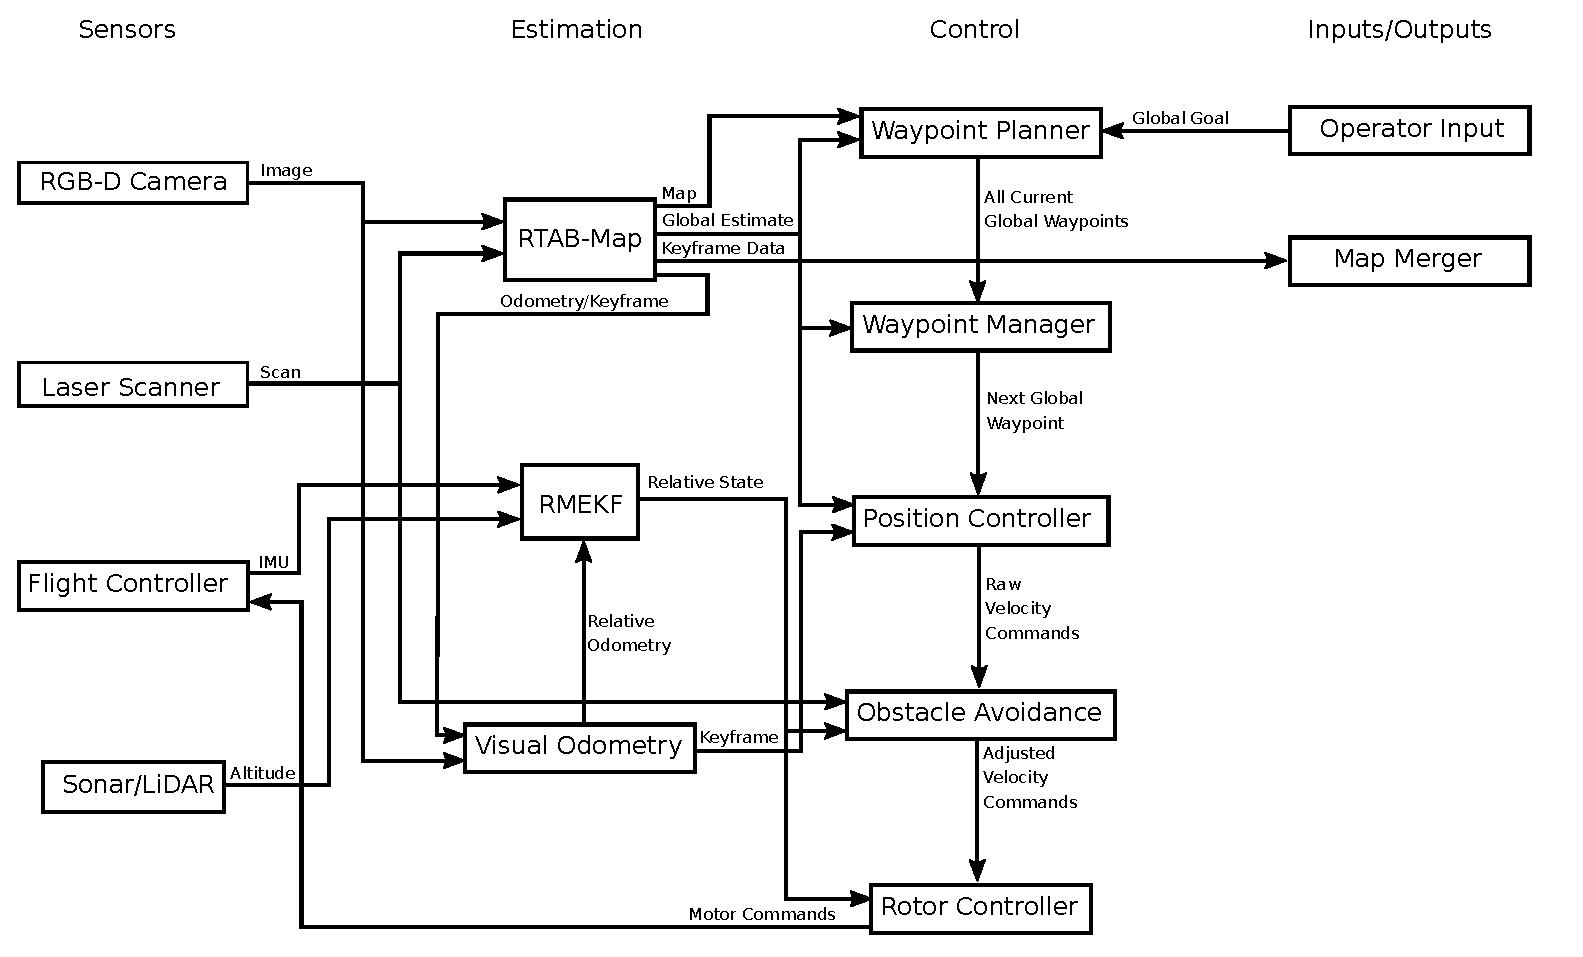
\includegraphics[width=1.0\linewidth]{rtab_relative_nav_network}
\caption{The network diagram of the relative navigation framework proposed in this paper}
\label{fig:rtab_network}
\end{figure*}

%%%%%%%%%%%%%%%%%%%%%%%%%%%%%%%%%%%%%%%%%%%%%%%%%%%%%%%%%%%%%%%%%%%%%%%%%%%%%%%%
\section{Planning}\label{planning}


\subsection{Global Goal Following with Relative Estimation}



\subsection{Reactive Path Planning}

%%%%%%%%%%%%%%%%%%%%%%%%%%%%%%%%%%%%%%%%%%%%%%%%%%%%%%%%%%%%%%%%%%%%%%%%%%%%%%%%
\section{Map Merging}\label{merge}

%%%%%%%%%%%%%%%%%%%%%%%%%%%%%%%%%%%%%%%%%%%%%%%%%%%%%%%%%%%%%%%%%%%%%%%%%%%%%%%%
\section{Results and Discussion}\label{results}
The designer is required to set many parameters for the genetic algorithm to work as derived in \cite{Parkinson2019}. The parameters we used, along with parameters specific to our implementation, are outlined in Table \ref{tab:parameters}.

%%%%%%%%%%%%%%%%%%%%%%%%%%%%%%%%%%%%%%%%%%%%%%%%%%%%%%%%%%%%%%%%%%%%%%%%%%%%%%%%
\section{Conclusions}\label{conclusions}

We were able to successfully generate paths with sufficient coverage to generate a high-fidelity map of the environment that do not appear to meander too much for a single UAV. Future work on this project will include improving the loop closure implementation to allow the algorithm to explore the design space better without getting caught in local minima. This will enable more efficient paths to be created. We expect the need to use the paths generated with a lower level path planner that can dynamically change waypoints according to obstacles and other unmapped disparities. Finally we plan to test the paths generated both in high fidelity simulation as well as in hardware.

%%%%%%%%%%%%%%%%%%%%%%%%%%%%%%%%%%%%%%%%%%%%%%%%%%%%%%%%%%%%%%%%%%%%%%%%%%%%%%%%

\bibliographystyle{IEEEtran} % We choose the "plain" reference style
\bibliography{mapping_paper_2019}

\end{document}
